\subsection{Datacrawler}
\label{Datacrawler}
The main goal of the datacrawler is to deliver the required datasets as specified in chapter \ref{sec:datasets}. The input to the datacrawler is simply a domain, which is provided by the ground truth. Depending on the configuration the output of the datacrawler can vary from a single screenshot (Section~\ref{DatasetVersion1}) to a complete graph of the given domain (Section~\ref{DatasetVersion2}).

The Section~\ref{datacrawler_requirements} will profoundly discuss the requirements in functionality for the datacrawler, which will serve as a basis for discussion for the decision between the frameworks \texttt{Puppeeter} and \texttt{Chromium Embedded Framework} (Section~\ref{datacrawler_framework_language}). Afterwards we will give an overview of the architecture (Section~\ref{datacrawler_architecture}) and highlight the idea of \textit{DataModules} in the crawler (Section~\ref{datacrawler_datamodulesystem}). Following that, we will discuss profoundly all developed \textit{DataModules} with their role in the Datacrawler and profoundly discuss the process of graph generation in Section~\ref{datacrawler_graph}.

In Section~\ref{datacrawler_scale} we will discuss how we successfully designed a sophisticated system to scale-out the Datacrawler reducing the total dataset creation time on Google Cloud Platform. Finally, in Section~\ref{datacrawler_results} we will dive into the final results and performance of the Datacrawler.

\subsubsection{Requirements}
\label{datacrawler_requirements}
The requirements in functionality for the datacrawler arise from the dataset specifications (Section~\ref{DatasetVersion1}, \ref{DatasetVersion2}) and our personal experiences. The next section will derive the requirements browser emulation, information accessibility, modularity and  scalability from the dataset specifications. Furthermore introduce programming language and native API access as additional requirements.

\paragraph*{Browser Emulation}
\label{browser_emulation}
One of the major requirements for the datacrawler is to find a convenient way of emulating a web browser. According to the dataset specifications, for every given website a screenshot $\tensorsym{I}$ has to be taken. In addition to that, every screenshot must represent the website as the user would see in a common browser. The latter and other attributes such as the loading time $l$ of a website like in a common browser make the emulation of a browser an inevitable requirement. 

\paragraph*{Information Accessibility}
\label{information_accessibility}
Accessing \textit{low-level} information such as the \textit{HTTP-Request} to change the \textit{user-agent} to generate a mobile screenshot $\tensorsym{M}$ or the \textit{Document Object Model (DOM)} to generate edges $a$ in the graph  is inevitable. The datacrawler has to be able to manipulate internal data structures and even able to inject own \textit{JavaScript-code} on the website.

\paragraph*{Modularity}
\label{modularity}
The datacrawler has to be as modular for allowing us to extend the datacrawler easily and decide which attribute should be calculated. This requirement in flexibility is raised from the fact that our dataset specifications might change over the time or new ones might be added.

\paragraph*{Scalability}
\label{scalability}
Both dataset versions require the analysis of at least 100,000 websites. Therefore, datacrawler has to be horizontally scalable to allow the analysis of multiple domains at once, and efficient in terms analysis time and start-up time. An inefficient and not scalable datacrawler would lead to multiple days of required analysis time and reflect also in high infrastructure costs.

\paragraph*{Programming Language}
\label{programming_language}
Since our team has a background software development in C++, we prefer a framework which allows us to write the Datacrawler in \texttt{C++}.

\paragraph*{Native API Access}
\label{native_api_access}
A non-native API access would lead to additional communication overhead, lead to performance issues and probably cut us in accessing low-level information. Therefore, we prefer a framework which offers a native API to access browser controls. 

\subsubsection{Framework}
\label{datacrawler_framework_language}
The previous section has shown some of the intricate requirements for the datacrawler. To answer those requirements in the given time frame, we investigated in frameworks, which would do most of the heavy-lifting for us such as networking, I/O or rendering of the website.

In our research we focused on the evaluation of frameworks, which base on the most common browser \texttt{Google Chrome} \cite{CommonBrowsers}. This section will investigate two frameworks \texttt{Puppeteer} and \texttt{Chromium Embedded Framework} (\texttt{CEF}) and discuss our decision for \texttt{CEF}. Both frameworks are providing an API to instrument the well-known browser \texttt{Chrome}.

\paragraph*{Puppeteer}
Our investigation whether \texttt{Puppeteer} (Section~\ref{puppeeter}) can be used in the Datacrawler has shown following results:

The requirement of \textbf{Browser Emulation}, since it is using an instance of \texttt{Chrome} to render websites. The requirement of \textbf{Information Accessibility}, due to functionalities in the domains DOM and Network. Furthermore \textbf{Modularity} is given per se by using \texttt{JavaScript} as the programming language, which makes the use of polymorphism possible as used in DataModule-System (Section~\ref{datacrawler_datamodulesystem}). The usage of \texttt{Chrome} ensures efficiency in terms of loading, rendering websites and retrieval of website information. Moreover, the combination of \texttt{Chrome} and \texttt{Puppeteer} can be scaled-out easily fulfilling the last requirement \textbf{Scalability} as described in Section~\ref{datacrawler_scale}.

Still \texttt{Puppeteer} fails to fulfill the requirement in \textbf{Programming Language } by providing only support for \texttt{JavaScript}. Moreover, due to the use of an HTTP-based RESTful API, \texttt{Puppeteer} clearly fails to offer native API access to browser controls, thus failing in the requirement \textbf{Native API Access}. 

\paragraph*{Chromium Embedded Framework}
Through the use of \texttt{Chromium Content API}, \texttt{CEF 3} provides a close integration between the browser and the host application including support for custom JavaScript objects and JavaScript extensions. Moreover, the host application is able to control resource loading, intercept the network, navigation and many more, while taking advantage of the same performance and technologies available in the \texttt{Google Chrome Web browser} \cite{CEFGeneralUsage}.

Therefore \texttt{CEF 3} clearly fulfills the requirement of \textbf{Browser Emulation} and \textbf{Information Accessibility}. Moreover, \textbf{Modularity} and \textbf{Scalability} is also given by using \texttt{C++} and the core functionalities of \texttt{Chromium}.

\texttt{CEF} clearly outperforms \texttt{Puppeteer} in the requirements \textbf{Programming Language} and \textbf{Native API Access} by providing native API access in \texttt{C++}.

\paragraph*{Framework Decision}
As Table~\ref{table_framework_decision} shows, both \texttt{Puppeteer} and \texttt{CEF} perform outstanding regarding our requirements. But still \texttt{Puppeeter} is outperformed by \texttt{CEF} in the requirements \textbf{Programming Language} and \textbf{Native API Access}. This leads to our decision to use \texttt{CEF} as our primary framework to build on.

\def\checkmark{\tikz\fill[scale=0.4](0,.35) -- (.25,0) -- (1,.7) -- (.25,.15) -- cycle;}
\begin{table}[h]
	\centering
	\begin{tabular}{lll}
		Requirement & \texttt{CEF}  & \texttt{Puppeeter} \\ \hline \hline
		Browser Emulation & \checkmark &  \checkmark  \\ \hline
		Information Accesibility &  \checkmark &  \checkmark  \\ \hline
		Modularity &  \checkmark &  \checkmark  \\ \hline
		Scalability &  \checkmark &  \checkmark  \\ \hline
		Programming Language &  \checkmark &   \\ \hline
		Native API Access &  \checkmark &    \\ \hline
	\end{tabular}
	\caption[Datacrawler requirements]{The table shows that both \texttt{Puppeeter} and \texttt{CEF} satisfy the framework requirements in browser emulation, information accessibility, modularity and scalability. But \texttt{Puppeteer} is clearly outperformed by \texttt{CEF} in programming language and native API access.}
	\label{table_framework_decision}
\end{table}

\subsubsection{Datacrawler Architecture}
\label{datacrawler_architecture}
One of the major points in the design and implementation of the Datacrawler was to meet the \textbf{Modularity} requirement (Section~\ref{modularity}). This led to the development of our sophisticated \textit{DataModule}-System and introduced the concept of \textit{Datamodules}.

Before diving into our implementation details by introducing the \textit{DataModule}-System, we will discuss how applications using \texttt{CEF 3} are build and work in general. Following that, we will introduce the \textit{DataModule}-System in great detail giving the required information to understand how \textit{Datamodules} work. Afterwards we will discuss how we take a screenshot of a website and tackle the challenge of detecting when a website has finished loading in the \textit{Screenshot}-Datamodule. Beyond that we will discuss how we take screenshots by emulating a mobile device and collect URLs by traversing the DOM. In the end we will show how we generate and output the graph (Section~\ref{datacrawler_graph}).

\paragraph*{CEF 3 Application Structure}
\label{datacrawler_cef_architecture}
\texttt{CEF 3} is based on multiple processes. It can mainly be divided into the \textit{browser}-process and \textit{render}-process.

\begin{itemize}
	\item The browser-process represents the host process of the application, which handles window creation, painting and network access. Furthermore, most of the application logic will run in the browser-process. 
	\item Multiple render-processes are responsible for rendering websites, executing JavaScript and running some application logic. Following the process model of \texttt{Chrome}, \texttt{CEF 3} spawns for every unique origin a render-process ensuring resource isolation, parallelism and better failure management.
\end{itemize}

The separate spawned processes communicate using \textit{Inter-Process Communication} (IPC). Application logic implemented in browser- and render-process can communicate by sending asynchronous messages as \textbf{URL-Datamodule} will show. Other processes are spawned when needed such as the \textit{plugin}-process for handling of plugins like \textit{Flash}.

In general \texttt{CEF 3} application consists of the class \texttt{CefApp} and \texttt{CefClient}. \texttt{CefApp} is responsible for process-specific callbacks such as returning handler for a custom render-process implementation. Whereas \texttt{CefClient} is responsible for handling browser-instance-specific callbacks such as returning handler for a customer website render implementation. It contains most of the application logic and is being used to create browser instances. As mentioned before, it can be used to control the browser-instance with custom implementation.

The following will briefly describe the start-up of an application using \texttt{CEF 3}:
\begin{enumerate}
	\item The \texttt{CefExecuteProcess}-method is used with custom implementation of \texttt{CefApp} to start separate processes. The application executable will be started multiple times representing new processes.
	\item \texttt{CreateBrowser} is used with custom implementation of \texttt{CefClient} to create a browser-instance. The browser instance is created in the browser-process, which means that there is only one browser at a time. Futhermore, an initial URL is passed to the browser-instance.
	\item In the implementation of \texttt{CefClient} \texttt{CefMessageLoop}-method is executed, which starts the event loop of the browser-instance. This means that browser-instance will start loading the given URL, handling network, rendering and many more. \texttt{CEF} takes care of spawning and using of existing render-processes.
	\item Once \texttt{CefQuitMessageLoop}-method is called, the message loop will be quit.
\end{enumerate}

\paragraph*{DataModule-System}
\label{datacrawler_datamodulesystem}
The naming of the DataModule-System derives from the purpose to bind, execute instances of Datamodules, collect results and output the dataset. The system consists of several components, which enable developers to implement and execute Datamodules independently increasing flexibility and reducing potential failures. In a plugin-and-play-manner developers can easily develop and add Datamodules to the Datacrawler.

The main idea of a Datamodule is to represent a single attribute in the dataset, which is calculated and added independently from other attributes to the dataset. In addition, each Datamodule can be individually configured and turned on or off by the user.

We are heavily utilizing polymorphism language feature of \texttt{C++} to enable previous mentioned features. Thus, a Datamodule consists of the implementation of the following interfaces:

\subparagraph*{\texttt{DataModuleBaseConfiguration}}
	This interface has to be implemented by each Datamodule. It is responsible for the creation and configuration of instances of a given Datamodule.


\subparagraph*{\texttt{DataModuleBase}}
	The DatamoduleBase-interface represents the core of each Datamodule. Most of application logic of the Datamodule will be implemented here.


\subparagraph*{\texttt{DataModuleBaseConfiguration}}
	This has to be implemented if the result of the Datamodule should be stored in the graph. It represents the results of the implemented Datamodule.\\
	
Figure~\ref{datacrawler_uml_diagram} represents a simplified UML-Diagram of the Datacrawler with the most important classes, interfaces and methods for understandig the DataModule-system. The figure does not show the implementation details of \texttt{CEF 3}, which are isolated and located in each Datamodule.

\begin{figure}
	\centering
	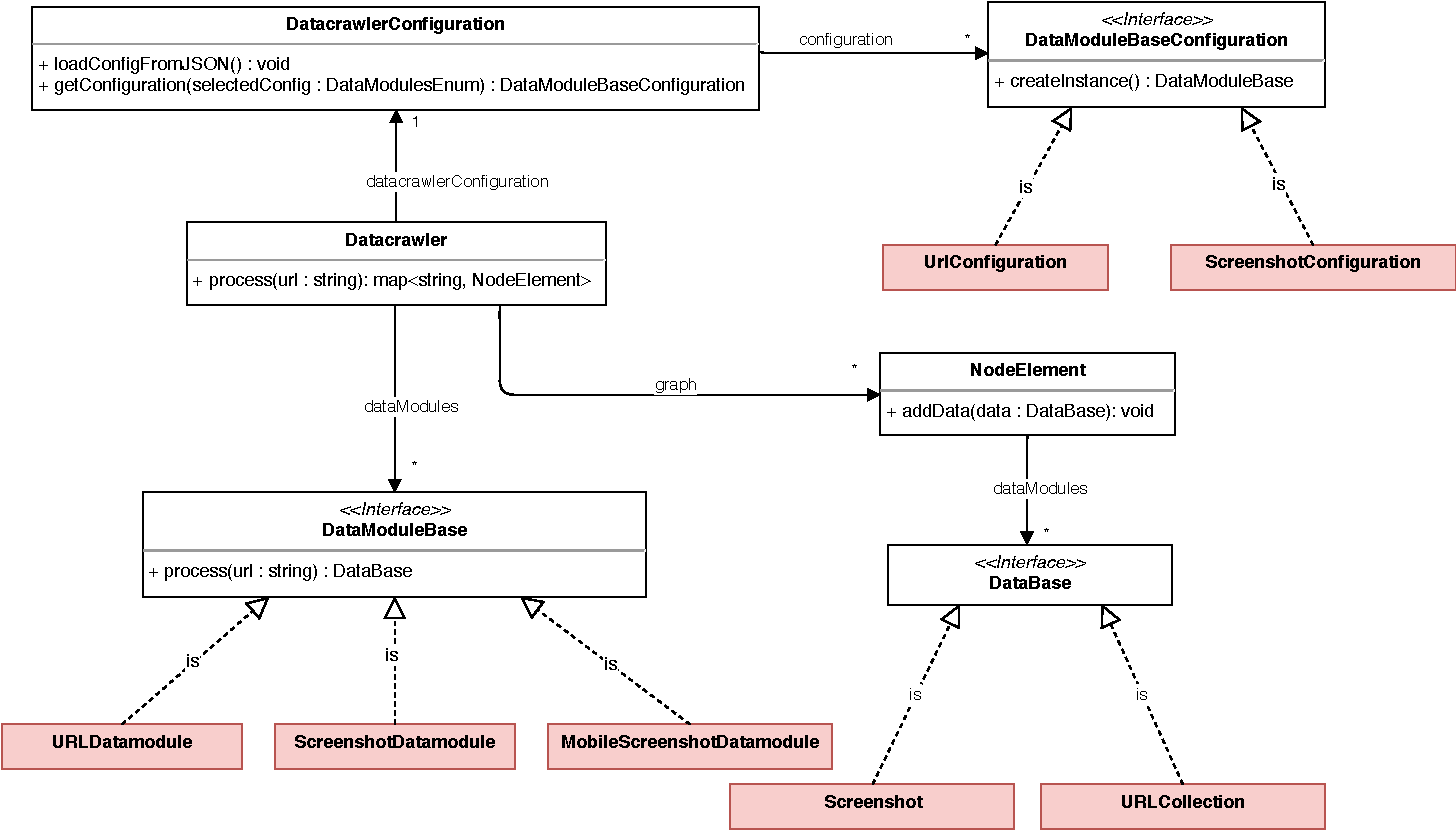
\includegraphics[scale=0.5]{resources/datacrawler_uml_diagram}
	\caption[UML-Diagram of the Datacrawler]{The figure shows the simplified UML-diagram of the Datacrawler with the most important classes and methods. Classes in the white boxes represent essential components of the DataModule-System such as the classes \texttt{Datacrawler}, \texttt{DatacrawlerConfiguration}, \texttt{NodeElement} and the interfaces \texttt{DataModuleBaseConfiguration}, \texttt{DataModulBase} and \texttt{DataBase}. Classes in the red boxes represent implementation of DataModules such as the \texttt{URLDatamodule}, \texttt{ScreenshotDatamodule} and \texttt{MobileScreenshotDatamodule}.}
	\label{datacrawler_uml_diagram}
\end{figure}

The class \texttt{Datacrawler} represents the entrypoint of the Datacrawler. It holds an instance of the class \texttt{DatacrawlerConfiguration}, which is responsible to load the user-defined Datamodules configuration using the method \texttt{loadConfigFromJSON()}. Upon successful loading, the Datacrawler creates instances of Datamodules using the method \texttt{createInstance()}. The interface method is implemented individually by each Datamodule reflecting custom Datamodule configuration. 

Once the \texttt{process(url)}-method has been called with an URL in \texttt{Datacrawler}, we create \texttt{NodeElement} representing the starting node and add it into our graph. Our graph is implemented as a key-value list, whereas the key represents the URL and the value our \texttt{NodeElement}-object. For dataset version 1 (Section~\ref{DatasetVersion1}) we assume to have a single node with a single screenshot. Afterwards we go through the our instantiated Datamodules and execute custom implementation of the method \texttt{process(url)}. At this point an isolated browser instance is created using \texttt{CEF 3}, which executes Datamodule-specific browser implementation. As soon as a Datamodule returns, we add the results to the current \texttt{NodeElement} and add \texttt{NodeElement} to our graph. 

Upon the completion of all Datamodules for a given URL, we add all generated edges of the Datamodule \texttt{URLDatamodule} into a FIFO queue in \texttt{Datacrawler}. In later sections we will discuss how and which URLs we select as edges of a node. Afterwards we repeat the process of creating a new object of \texttt{NodeElement}, executing of Datamodules, adding the results into new \texttt{NodeElement} and URLs to our FIFO queue for the oldest entry. We skip a given URL if there is a key-value pair in our list or if we reach our maximal number of nodes in the graph.

\begin{figure}
	\centering
	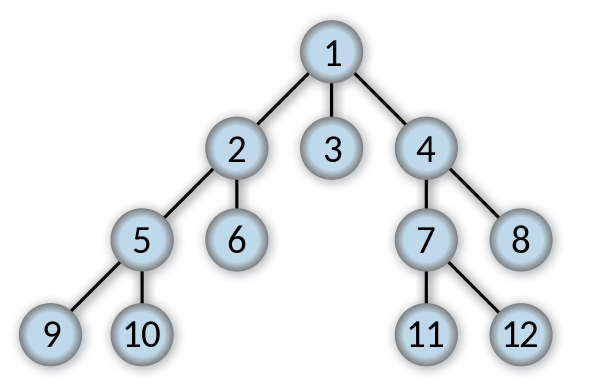
\includegraphics[scale=0.35]{resources/breadth-first}
	\caption[Illustration of the Breadth-First-Search Algorithm]{ The numbers in the nodes show the order in which nodes are expanded in breadth-first search. It shows that all nodes reachable from a selected nodes are expanded, before selecting the first node encountered and expanding the nodes reachable from it. E.g the selected node is \textbf{1} and the nodes \textbf{2}, \textbf{3} \textbf{4} are expanded, before we select \textbf{2} and expand the node \textbf{5} and \textbf{6}.}
	\label{datacrawler_breadth_search}
\end{figure}

The use of the FIFO queue leads to breadth-first search in our graph in opposition to a deep search, which is implemented using a LIFO queue. The breadth-first search means that we expand all nodes reachable from the edges of our current node and selecting the oldest entry as new node, rather than using the first edge, expanding the reachable node and selecting it as the current node. By using the breadth-first search, we maximize the number of directly reachable nodes from a given node. This leads to a wide and dense rather than deep and sparse graph. We perform a breadth-first search because we prefer to have connections between those nodes rather than having long strings originating from a root node. That way we capture at least some of the page-internal linking structure. Figure~\ref{datacrawler_breadth_search} illustrates the breadth search exemplary.

\paragraph*{Screenshot-Datamodule}
\label{datacrawler_screenshot_datamodule}
The Screenshot-Datamodule is responsible for visiting a website by a given URL and taking a screenshot upon successful loading as specified in Section~\ref{DatasetVersion1}. The entrypoint of the Datamodule is \texttt{process(url)}-method in \texttt{ScreenshotDatamodule}-class. Upon completion, the Datamodule returns an instance of \texttt{Screenshot}, which contains a screenshot and information about width and height of the screenshot.

In general the Screenshot-Datamodule addresses three difficult problems with the help of \texttt{CEF 3}: 

\begin{enumerate}
	\item \textbf{Any} website given by URL  has to be loaded without exceptions.
	\item \textbf{Every} website has to be rendered in a format to take a screenshot from.
	\item The Datamodule has to detect when a given website has finished loading to take a screenshot.
\end{enumerate}

The following sections will profoundly discuss how the Screenshot-Datamodule successfully addresses previous mentioned problems with the use of \texttt{CEF 3}:

\subparagraph*{Loading} 
The Screenshot-Datamodule consists of \texttt{ScreenshotDatamodule} and implementations of the interfaces \texttt{CefClient} and \texttt{CefRenderHandler}. In \texttt{process(url)}-method of \texttt{ScreenshotDatamodule} a synchronous browser instance is created with our implementation of \texttt{CefClient} and the given URL. As mentioned earlier \texttt{CefClient} is responsible for browser-instance-specific callbacks and hence the place to customize the browser for our needs. Therefore, we implement \texttt{CefClient} and overwrite the method \texttt{GetRenderHandler()} to return a custom implementation of \texttt{CefRenderHandler}. The browser instance will now use our implementation of \texttt{CefRenderHandler} to paint the website during loading.

The use of a synchronous browser instance allows us to iterate through the event loop of the browser instance by ourselves until we take a screenshot of the given website. This is mandatory for both threads, which are created directly after the browser instance and play a critical role in detecting if a website has finished loading. 

\subparagraph*{Rendering}
In the world of \texttt{Chromium} \textit{rendering} relates to the process of parsing, transforming of website data to generate DOM, executing JavaScript, applying CSS and painting of the website. 

In Screenshot-Datamodule the interface \texttt{CefRenderHandler} is not responsible for rendering a website, but only for the painting to the end user device. In our implementation, we have implemented the \texttt{GetViewRect()} and \texttt{OnPaint()}-method of \texttt{CefRenderHandler}. Latter is the place to paint the website to the end user device, whereas we define in \texttt{GetViewRect()} the height and width of the output from the browser. In case of \texttt{CEF 3} the \texttt{OnPaint()}-method is invoked each time if the browser instance detects invalidation caused by changes in the DOM and CSS. These changes can be caused by a loading website, animations or dynamically changing content due to custom JavaScript code.

In each invocation of \texttt{OnPaint()} following information are passed as parameters:

\begin{itemize}
	\item Reference to the current browser instance.
	\item Reference to the buffer, where image information are kept about the website.
	\item Information about the height and width of the given website.
\end{itemize}

The buffer is an array of respectively one byte encoded single characters, where each character is representing a channel of the color space \texttt{BGRA}. Consequently, a single pixel corresponds to four characters in the buffer. The array represents the pixels from the left most to the right most starting from the top of the viewport in repeating order of the color space. Thus, the buffer itself contains only information about visible area as defined in \texttt{GetViewRect()}, which reflects the viewport of the browser.

On each invocation we allocate total of $4 * \texttt{width} * \texttt{heights}$ bytes in the memory and copy the content of our buffer into it. Once we detect the website has finished loading, we can access the latest painting of \texttt{OnPaint()} from the memory.

\subparagraph*{Detection}
\label{datacrawler_detection}
In our current implementation the browser instance calls \texttt{OnPaint()}-method to update the view port, whenever a change occurs on the website. In practice this means that our implementation might return screenshots of partially loaded websites, if we access to the buffer at a bad time. The simple solution to wait a given time $t$ and take the most recent screenshot is not an option. This static approach would lead to high analysis time per website and violate the scalability requirement (Section~\ref{scalability}). We have to detect, when a given website has finished loading to reduce our analysis time per website.

In general, there are multiple states during the loading of a website, which can be interpreted that a given website has finished loading. Before we discuss our approaches to tackle this complex problem, we define our understanding when a website has finished loading:

\begin{center}
	\textit{A website has finished loading, if and only if all elements are painted on the view port and no new elements are being painted.}
\end{center}

Our definition includes the painting and rendering of the given website in the browser and represents the \textit{natural} behavior of a browser. The following definition does not include those aspects:

\begin{center}
	\textit{A website has finished loading, if and only if all the content of the website has been downloaded successfully from the internet.}
\end{center}

Based on our assumption we have developed two algorithms for this problem:

\begin{itemize}
	\item Detection based on calculation of \textit{change} matrices. 
	\item Detection based on \texttt{OnLoadingStateChange()}-method of \texttt{CEF 3} and hard coded waiting time.
\end{itemize}

Our algorithm based on calculation of change matrices, assumes that the number of changed pixels per screenshot will dramatically reduce over time. In other words, given the screenshots $I_{t}, I_{t+1}, I_{t+2}\in \{0, ... , 255\}^{width\times height \times 4}$ taken at times $t$, $t+1$,  and $t+2$ respectively, the total number of changed pixels  $|\Delta_{t,t+1}|$ between $I_{t}$ and $I_{t+1}$ will be less than $|\Delta_{t+1,t+2}|$. Furthermore, we assume that the $|\Delta|$ will converge for $t \rightarrow \infty$ meaning that the website has finished loading. The blue line in Figure~\ref{plot_assumption_number_changes} illustrates our assumption exemplary.

In order to calculate the number of changed pixels between two screenshots $I_{t}$ and $I_{t+1}$, we have introduced the change matrix $C_{t,t+1} \in \{0,1\}^{width\times height}$. Each element $c_{i,j} \in C_{t,t+1}$ represents the change state between the pixels $\mathbf{s}^{t}_{i,j,} \in I_{t}$ and $\mathbf{s}^{t+1}_{i,j,}  \in I_{t+1}$, which in turn are in $\{0, ... , 255\}^{4}$ representing the color space \texttt{BGRA}.

On every invocation of \texttt{OnPaint()} we calculate the change matrix $C_{t,t+1}$ on basis of the current screenshot $I_{t+1}$ and the screenshot $I_{t}$ of the previous invocation. The following applies for each element $c_{i,j} \in C_{t,t+1}$ :

\[
c_{i,j} =
\begin{cases}
1,& \text{if $\mathbf{s}^{t}_{i,j,} \neq \mathbf{s}^{t+1}_{i,j,}$ } \\
0,              & \text{otherwise}
\end{cases}
\]

We compute the total number of changes from $I_{t}$ to $I_{t+1}$ with $|| C_{t,t+1}||$ and save it in every invocation of \texttt{OnPaint()} for later use. In addition, we also calculate the maximum number changes per screenshot with $width \times height$ and call it $C_{MAX}$. The red line for \texttt{nationalgeographic.com} in Figure~\ref{plot_assumption_number_changes} shows that the number of changes is indeed converging, but not stable as expected. We take this into account and calculate on every invocation the average $C_{AVG}$ for the number of changes at $t-n, t-n+1, ..., t$, whereas $n$ is defined in the Datamodule configuration and $t$ represents our current screenshot. Putting everything together we detect if a given domain has finished and take a screenshot by following equation is true:

\[
{\frac{C_{\text{AVG}}}{C_{\text{MAX}}} \leq p_{C}; \quad   {\frac{C_{\text{AVG}}}{C_{\text{MAX}}}}, p_{\text{C}} \in [0,1]}
\]

The fraction ${\frac{C_{\text{AVG}}}{C_{\text{MAX}}}}$ describes the average in percentage of changes over the last $n$ screenshots and $p_{C}$ is the user-defined threshold. 

Furthermore, we have observed that for websites such as \texttt{timodenk.com} the \texttt{OnPaint()}-method is only called for a limited number of times. This might not be enough to leverage our detection algorithm. Therefore we have implemented a thread, which starts upon every \texttt{OnPaint()}-invocation a timer. The timer has the goal to return a screenshot, if \texttt{OnPaint()}-method has not been invoked for the user-defined time.  

\begin{figure}
	\centering
	
	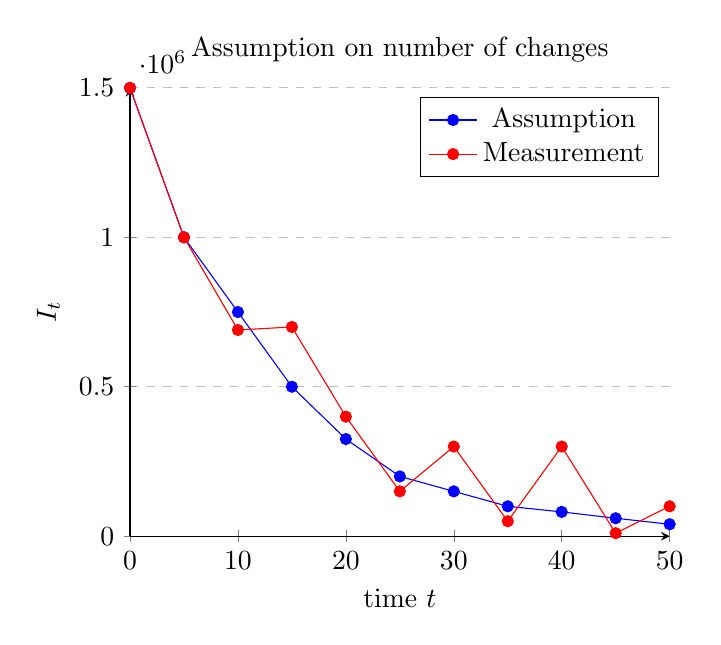
\begin{tikzpicture}
	\begin{axis}[
	title={Assumption on number of changes},
	axis lines = left,
	xmin=0, xmax=50,
	ymin=0, ymax=1500000,
	xlabel = time $t$,
	ylabel = {$I_t$},
	ymajorgrids=true,
	grid style=dashed,
	]
	%Here the blue parabloa is defined
	\addplot[
	color=blue,
	mark=*,
	]
	coordinates {
		(0,1500000)(5,1000000)(10,750000)(15,500000)(20,325000)(25,200000)(30,150000)(35,100000)(40,81250)(45,60000)(50,40000)
	};
	\addplot[
	color=red,
	mark=*,
	]
	coordinates {
		(0,1500000)(5,1000000)(10,690000)(15,700000)(20,400000)(25,150000)(30,300000)(35,50000)(40,300000)(45,10000)(50,100000)
	};

	\addlegendimage{/pgfplots/refstyle=plot_1_y1}\addlegendentry{Assumption}
	\addlegendimage{/pgfplots/refstyle=plot_1_y2}\addlegendentry{Measurement}
	\end{axis}
	\end{tikzpicture}
	\caption[Figure on Total Number of Changes on a Website]{The figure illustrates in blue our assumption regarding the number of total changes $|| C_{t,t+1}||$ from $I_{t}$ to $I_{t+1}$. It shows that the number of total changes dramatically reduce and converge for $t \rightarrow \infty$. The red line illustrates the actual measured number of changes for \texttt{nationalgeographic.com} with the resolution $1920$ in width and $1080$ in height. }
	\label{plot_assumption_number_changes}
\end{figure}

Our second algorithm implements \texttt{OnLoadingStateChange()}-method of \texttt{CefLoadHandler}, which will be invoked upon a website has been loaded successfully. During invocation the parameter \texttt{isLoading} is passed, which is true if the given website has been loaded and false if not. However, this variable does not indicate that the given website has been painted successfully. It only indicates the browsers is ready to paint the given website. Therefore we have implemented a timer, which will start upon \texttt{isLoading} is true, run for a user-defined time and return the content of the buffer.

In addition both algorithms implement a thread, which starts a timer upon the loading of a website. This timer represents a hard timeout for the Screenshot-Datamodule and will run for a user-defined time. After timeout it will ultimately return a screenshort. Thus, guaranteeing us to return the buffer  in any circumstances.

\begin{table}
	\centering
	\begin{tabularx}{\textwidth}{l l l l l l}
		Algorithm based on & Partially Loaded & Fully Loaded & \%  & Total \\ \hline \hline
		change matrices & 13 & 87 & 13 & 100 \\ \hline
		\texttt{OnLoadingStateChange()} & 3 &  97 & 3 & 100
	\end{tabularx}
	\caption[Performance of algorithms for detection of website finished loading]{The table illustrates the performance of our algorithms based on change matrices and \texttt{OnLoadingStateChange()} for the top 100 websites from \texttt{Open PageRank}. The websites are manually evaluated by us. A website is categorized as partially loaded, if it is obviously missing parts of the website, and fully loaded, if not. The approach using \texttt{OnLoadingStateChange()} performs with $3\%$ of partially loaded websites better than our approach with change matrices with $13\%$. }
	\label{table_compare_algorithm_screenshot}
\end{table}

We have manually evaluated both approaches using the top 100 website in \texttt{Open PageRank} (Section~\ref{OpenPageRank}). Our results are described in Table~\ref{table_compare_algorithm_screenshot}. They show that the algorithm based on \texttt{OnLoadingStateChange()} outperforms the algorithm based on change matrices. This ultimately leads to our decision to use \texttt{OnLoadStateChange()} as our preferred detection algorithm.

\paragraph*{MobileScreenshot-Datamodule}
\label{datacrawler_mobilescreenshot_datamodule}
The MobileScreenshot-Datamodule is responsible for visiting a website by a given URL and taking a screenshot upon successful loading. The \texttt{process(url)}-method is the entrypoint for the Datamodule. In contrast to the Screenshot-Datamodule, the visited website has to be in mobile resolution and mobile view leading to a screenshot taken from a mobile device (Section~\ref{DatasetVersion2}).

In total there are two ways to request a mobile view for a website:

\begin{itemize}
	\item Visit the website with mobile device resolution e.g $375$ in width and $667$ in height
	\item Declare the \textit{user-agent} as a mobile device e.g  \texttt{Mozilla/5.0 (iPhone CPU)}
\end{itemize}

While the resolution represents the size of the view port in which the given website is being displayed, the user-agent represents the identification of the browser. It is a request header containing a characteristic string that allows the communication partner to identify application type, operating system, software vendor and version of the requesting browser instance. The request header is being send on every HTTP method such as \texttt{GET}. The \texttt{CEF 3} uses a desktop user-agent per default as Figure~\ref{compare_resolution} shows.

Our initial assumption, that requesting a website with mobile resolution would lead to a mobile view, was right for a majority of the websites. But Figure~\ref{compare_resolution_useragent} shows that there are exceptions such as \texttt{youtube.com}, where it is not enough to scale down the resolution. Hence, we consider in our implementation to use a mobile resolution and user-agent. While we reuse most of the implementation of the Screenshot-Datamodule such as the loading, rendering and detection, we extend and change the implementation at specific points to support mobile view.

First we adjust the resolution of the browser instance in \texttt{GetViewRect()} to mobile resolution, which is given by the mobile screenshot requirement described in dataset version 2 (Section~\ref{DatasetVersion2}). Second, we intercept all outgoing requests from the browser instance and add the required mobile user-agent header. This is done by providing a custom implementation of the interface \texttt{CefRequestHandler} having the primary goal to handle browser requests. In \texttt{CefRequestHandler} we implement the \texttt{OnBeforeResourceLoad()}, which is invoked every time before a request is send. During invocation the outgoing request \texttt{CefRequest} is passed as parameter, which allows us to modify the request for our needs. The request contains beside the body, target URL, HTTP method also a key-value store representing the header section of the request. Upon every invocation we modify the key-value store and overwrite the key \texttt{User-Agent} with the value \texttt{Mozilla/5.0 (iPhone [...]) Chrome/71 [...] Mobile [...]}. The latter represents the Chrome browser on the mobile device \texttt{Apple iPhone}. 

The interception and modification led us to successfully emulate a mobile device from our Datacrawler, allowing us to take screenshots from a mobile device.

\begin{figure}
	\centering
	\begin{subfigure}{0.6\textwidth}
		\centering
		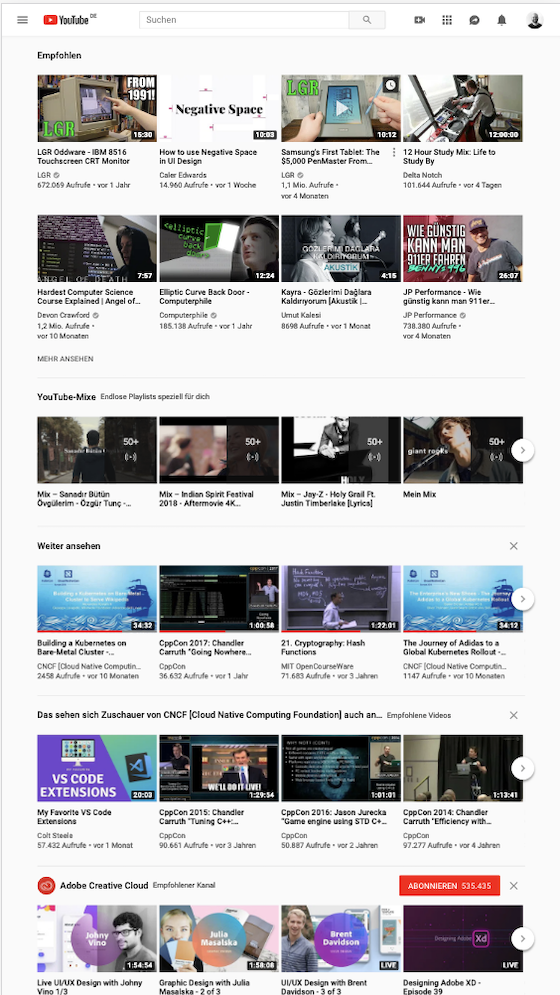
\includegraphics[width=0.5\linewidth]{resources/screenshot_resolution}
		\caption{}
		\label{compare_resolution}
	\end{subfigure}%
	\begin{subfigure}{0.6\textwidth}
		\centering
		
\includegraphics[width=0.5\linewidth]{resources/screenshot_resolutionanduseragent}
		\caption{}
		\label{compare_useragent}
	\end{subfigure}
	\caption[Mobile and Desktop Screenshot taken by the Datacrawler]{Two screenshots taken from the website \texttt{youtube.com}. The figures (a) and (b) were taken with a browser instance having the resolution $375 \times 667$. In addition, we changed the user-agent of the figure (b) to represent a mobile device and use the default user-agent of \textit{CEF 3}. The usage of the mobile user-agent clearly shows that the website is being displayed for mobile devices in figure (b), whereas in figure (a) not.}
	\label{compare_resolution_useragent}
\end{figure}

\paragraph*{URL-Datamodule}
\label{datacrawler_url_datamodule}
The URL-Datamodule represents one of the most complex Datamodules in the Datacrawler. It is responsible for returning a set of valid URLs for a given website, server and client errors occurred during loading, title, loading time and download size of the website. While calculating and returning so many attributes in a single Datamodule is contrary to the principles of the Datamodule-System, we had to do the trade-off in order to (1) reduce overall development and (2) analysis time. The latter arises from the fact that for every single attribute we have to create a new browser instance and reload the entire website, which takes a tremendous amount of computing resources and time. Thus, complexity URL-Datamodule arises by calculating multiple attributes at once and the usage of different processes and their communication based on \textit{IPC}.

In general, the URL-Datamodule is executed by invoking the \texttt{process(url)}-method. Upon successful completion it returns an instance of \texttt{URLCollection}, which is added to \texttt{NodeElement} and contains previous mentioned attributes. Similar to other Datamodules, we implement \texttt{CefClient} and other interfaces with our custom implementation and start a browser instance for the given URL. In the following, we will profoundly discuss the implementation by discussing each attribute calculation solely.

\subparagraph*{URLs}
The URL-Datamodule has to return valid URLs. This attribute is specified as following in the specification of dataset version 2 (Section~\ref{DatasetVersion2}):

\begin{center}
	\textit{Each edge $a$ represents a possible navigation from web page $v_1$ to $v_2$ [...] and has the same Fully Qualified Domain Name.}
\end{center}

According to the specification a given URL is only valid if it is a possible navigation and has the same FQDN. Possible navigation means that only URLs found as a \texttt{href}-attribute in \texttt{<a>}-tags in the \texttt{HTML}-code of the website can be considered as valid. This follows from the fact that in \texttt{HTML} \texttt{<a>}-tag is the only tag, which allows the user to navigate to other pages from the current viewed page. While possible navigation describes where to find valid URLs, equality in FQDN describes which URLs to choose from a set of URLs.
For example the FQDN for the URL \texttt{http://web.samedguener.com/index.html} is \texttt{web.samedguener.com}. While the URL \texttt{http://web.samedguener.com/conta-
ct.html} found on the website is a valid with \texttt{web.samedguener.com} as FQDN, \texttt{http://samedguener.com/} is not with \texttt{samedguener.com}.

In general, all browsers have a common process to render a website: They download the source code of the requested webpage, parse and build the DOM. The DOM is built and represented as a tree, where nodes are \texttt{HTML}-tags and children of a node represent nested \texttt{HTML}-tags. In \texttt{CEF 3}, we are able to directly access the DOM after a website has finished rendering. 

While \texttt{isLoading}-parameter of \texttt{OnLoadingStateChange()}-method in \texttt{CefLoadHandler} is used for detecting if a given website has finished rendering, the DOM itself can be accessed by implementing \texttt{Visit()}-method of \texttt{CefDOMVisitor}.
Due to the nature of the DOM being built in the render-process, \texttt{CefDOMVisitor} has to be run in the render-process conversely to \texttt{CefLoadHandler} and all other implementations running in the browser-process. Therefore, we implement \texttt{OnMessageReceived()} of \texttt{CefRenderProcessHandler} respectively running the the render-process to run an instance of \texttt{CefDOMVisitor}. The \texttt{OnMessageReceived()}-method is invoked if the render-process receives any IPC-message from any other process. \texttt{CefRenderProcessHandler} is responsible for handling render-process-specific implementations. The user can change the default behaviour by implementing this interface. Moreover, we implement also \texttt{OnMessageReceived()}-method in \texttt{CefClient} to receive IPC-messages from the render-process.

Having all important components together, this leads to the following workflow of the URL-Datamodule:

\begin{enumerate}
	\item Custom implementation of \texttt{CefRenderProcessHandler} is passed to \texttt{CefApp} during \texttt{CEF 3} initialization.
	\item In URL-Datamodule a browser instance is created and started with custom \texttt{CefClient} implementation returning the \texttt{CefLoadHandler} implementation.
	\item Upon successful \texttt{OnLoadingStateChange()} in \texttt{CefLoadHandler}, send an IPC-message to the render process ultimately invoking \texttt{OnMessageReceived()} in \texttt{CefRenderHandler}
	\item Create instance of custom implemented \texttt{CefDOMVisitor} and execute application logic.
	\label{point_implement_cefdomvisitor}
	\item Upon successful URL gathering, send an IPC-message with collected URLs to browser-process invoking ultimately \texttt{OnMessageReceived()} in \texttt{CefClient}. Then, return the results as Datamodule to the Datacrawler.
\end{enumerate}  

During the execution of \texttt{OnMessageReceived()} in \texttt{CefRenderProcessHandler} we use the passed browser instance to execute our implementation of \texttt{CefDOMLoader} against it (Section~\ref{point_implement_cefdomvisitor}). The main application logic is then executed in \texttt{Visit(CefDOMDocument)}-method of \texttt{CefDOMVisitor}. The passed argument \texttt{CefDOMDocument} represents the DOM of the current visited website. Since the DOM is organized as a tree, we use the breadth-first search (Section~\ref{datacrawler_breadth_search}) for tree traversal, check each if given node is a \texttt{<a>}-tag and retrieve the URL from the \texttt{href}-attribute and the URL text if given. Upon retrieval we filter the URLs having the same FQDN using several regular expressions and create respectively objects of the class \texttt{URL}. In addition, we use regular expression to detect whether the given URL has \texttt{HTTPS} enabled and enrich the \texttt{URL} object with this information. In the end, we return a list of \texttt{URL} objects to the URL-Datamodule.

\subparagraph*{Loading Time}
\texttt{OnLoadingStateChange()} in \texttt{CefLoadHandler} is invoked if the website transitions between loading states such as from not being loaded into being loaded or from being loaded into finished loading. To track the loading time of the given website, we just stop the time between both transitions and calculate the delta. We return the loading time back to the URL-Datamodule upon \texttt{CefDOMVisitor} has returned the valid URLs.

\subparagraph*{Client and Server Errors}
During the loading of a website, the Datacrawler can face client- and server-side errors. On the one hand client-side errors are e.g connection timeout, connection interruption, endless redirection or an invalid TLS certificate. They occur if no successful connection to the website could be established at all. On the other hand server-side errors are returned by the server and redirected through the browser instance to the end-user. They occur if a connection to the server is successful, but the given resource is e.g not accessible. Server-side errors are \texttt{HTTP} status codes such as \texttt{404} for \texttt{resource not found}. 

In general client-side errors can be obtained by implementing \texttt{OnLoadError()}-method in \texttt{CefLoadHandler}. It is invoked if no connection could be established to the server at all. Server-sided errors can be obtained by implementing \texttt{OnLoadEnd()}-method in \texttt{CefLoadHandler}. Since only client-side error or server-side error can happen at once, only one of the methods is invoked. After invocation we save the client-server or the server-side error and return it to the URL-Datamodule.

\subparagraph*{Title}
The title of the website can be accessed by implementing \texttt{OnTitleChange()}-method of \texttt{CefDisplayHandler}, which is mainly responsible in handling the display state of the browser e.g browser switching to fullscreen mode. The custom implementation of \texttt{CefDisplayHandler} is then passed to \texttt{CefClient}. Due to the fact that \texttt{OnTitleChange()}-method is invoked everytime the title of a website changes, we only use value of the initial invocation and pass it directly to the URL-Datamodule.

\subparagraph*{Download Size}
As specified in the dataset version 2 (Section~\ref{DatasetVersion2}) the download size of a website represents the total amount of data downloaded during the loading of a website. In general, the process of loading a website consists of sending requests to a webserver and receiving responses over the internet. In our case, the total number of bytes received in the responses represents the download size of a website.

\texttt{CEF} allows us to intercept the raw received responses before they are processed in the render-process of the browser. By implementing \texttt{filter()}-method of \texttt{CefResponseFilter} we add a \textit{filter} which receives the response beforehand, reads the number of bytes received and forwards the response to the browser-instance. In general, \texttt{CefResponseFilter} is returned by an instance of \texttt{CefRequestHandler}, which is passed to \texttt{CefClient}. Before we return the gathered valid URLs from the URL-Datamodule to the Datacrawler, we convert the download size to kilobytes and return it with the other attributes to the Datacrawler.

\subsubsection{Generating the Graph}
\label{datacrawler_graph}
As specified in dataset version 2 (Section~\ref{DatasetVersion2}), for each passed domain to the Datacrawler, we have to output a graph with nodes enriched by information from the Datamodules. Before we delve into the concrete implementation of graph generation process, we will profoundly discuss the output format of the graph, which is later consumed by our machine learning model.

\paragraph*{Graph Data Format}
We run for each given domain an independent Datacrawler instance. This means that upon successful completion of the Datacrawler, we will have only printed out exactly one graph belonging to the passed domain. Following this, we create an own folder for the computed domain and name the folder after the rank found in the Open PageRank (Section~\ref{OpenPageRank}). The graph itself is represented by a file in the \texttt{json}-format and named after the rank in Open PageRank. While most of the dataset information can be found in the \texttt{json}-file, we save our screenshots for the domain in the folder called \texttt{img}. We differ between normal and mobile screenshots by adding the suffix \texttt{\_mobile} to the name of the mobile screenshots. Furthermore, we number consecutively each image according an internal ID specified for each node in the \texttt{json}-file.

The \texttt{json}-file consists of an array containing nodes represented as \texttt{json}-objects. Each \texttt{json}-object consists mainly of attributes calculated by the URL-Datamodule. Furthermore, each node has an array containing the URLs representing the edges of the given node. We have to emphasize that only URLs has been taken into account, which are also represented as nodes in the graph. Listing~\ref{lst:examplecom_graph} exemplary shows the graph for \texttt{example.com}.

\begin{lstlisting}[language=json,firstnumber=1,label={lst:examplecom_graph},
    language=Python,
    caption={[Example Graph generated by the Datacrawler]Graph output for the domain \texttt{example.com}. The graph nodes are \texttt{json}-objects in the root array of the \texttt{json}-file. The \texttt{baseUrl}-attribute shows affiliation of the node to the given URL. Futhermore, each \texttt{json}-object consists of attributes mainly calculated in the URL-Datamodule such as client-sided and server-sided error (here: \texttt{client\_status} and \texttt{server\_status}), loading time, size and finally the valid URLs with the URL text. In general, all URLs found in the nodes are represented as nodes in the graph. Finally, each computed URL has an ID assigned, which represents respectively the name of the screenshots for the URL.},
    captionpos=b]
[{
	"id": 1,
	"baseUrl": "https://example.com",
	"client_status" : null,
	"loading_time": 8822,
	"server_status": 200,
	"startNode": true,
	"size": 1222,
	"title" "example.com",
	"urls": [
		{
			"url": "https://example.com/2",
			"url_text": "Second Page"
		},
	...
	]
	},
	{
	"id": 2,
	"baseUrl": "https://example.com/2",
	"startNode" : false,
	...
}]
\end{lstlisting}

\paragraph*{Process of Graph Generation} 
The process of the graph generation is done in the \texttt{Datacrawler}-class and \texttt{GraphOutput}-class, which are responsible for the graph calculation and outputting of the graph to the local disk. In general the nodes of the graph are saved in a key-value data structure, where the key is the URL of the computed node and the value represents an object of type \texttt{NodeElement} (Section~\ref{datacrawler_architecture}). \texttt{NodeElement} consists of a simple list of the type \texttt{DataBase} representing attributes calculated by the Datamodules such as screenshots or URLs.

Upon the invocation of \texttt{process(url)}, the Datacrawler creates the initial \texttt{NodeElement}, runs all registered Datamodules against the passed domain and adds the results of the Datamodules to the node. Afterwards retrieved URLs of the current node are accessed and put into a working queue for further computation by the Datacrawler. Then, we recursively repeat the process for all elements in the queue until the graph has reached the limit of 8 nodes as specified in dataset version 2 (Section~\ref{DatasetVersion2}). Before we hand over the graph to \texttt{GraphOutput} for outputting it to local disk, we have to remove edges from the node which direct to no nodes in the graph. This done by going through all the edges of a node and checking whether the given URL as key is mapped to a node. If it is not mapped to a key, we remove the edge.

Upon the removal of arbitrary edges in the graph, we pass our key-value list to \texttt{GraphOutput}. Then for each element of the list, we calculate the \texttt{json}-object by going through each element of \texttt{Database} in \texttt{NodeElement} and generate the attribute entry. Afterwards we add the \texttt{json}-object to \texttt{json}-array and continue. For the subtype \texttt{Screenshot} of \texttt{Database}, we use \texttt{OpenCV} to output respective screenshots of the current node. We scale down mobile screenshots by factor two and desktop screenshots by factor four. Finally, the screenshots are outputted in \texttt{JPEG}-format with \texttt{CV\_IMWRITE\_JPEG\_QUALITY} set to 75 out of 100, where the more represents a better quality of the screenshot. 

\subsubsection{Running the Datacrawler at Scale}
\label{datacrawler_scale}
It is not sustainable to run the processing sequentially on a single Datacrawler instance. This section will profoundly discuss how we successfully managed to dramatically reduce the analysis time to $28$ hours by scaling the Datacrawler using Kubernetes on Google Cloud Platform. 

The next section will discuss the experiment we did to get a rough estimate of the processing time for dataset version 2. Afterwards we will discuss the general system design we created to scale the Datacrawler. We will focus on how we leveraged \texttt{redis} as working queue to distribute domains to be analyzed among the Datacrawler instances and used a network file system to collect the results from all Datacrawler instances. Finally we will delve into the Datacrawler container and discuss how consume work items with the Datacrawler from our queue.

\paragraph*{Processing Time}
\label{datacrawler_processing_time}
For scaling the Datacralwer to process the tremendous amount of $100,000$ domains and generate the dataset version 2, we had to do track the average processing time and required disk space for each domain beforehand.

For this purpose we run the final version of the Datacrawler for the following $12$ hand-selected domains: \texttt{sap.com}, \texttt{google.com}, \texttt{samedguener.com}, \texttt{timodenk.com}, \texttt{twitter.com}, \texttt{facebook.com}, \texttt{nationalgeographic.com}, \texttt{youtube.-
com}, \texttt{tagesschau.de}, \texttt{cnn.com.tr}, \texttt{nytimes.com}, and \texttt{pornhub.com}

We run the experiment using one Datacrawler instance on a single CPU clocked at $2.3$ Ghz on \texttt{Ubuntu 16.04}. Furthermore, we provide the Datacrawler with $500$ Mb of RAM, enough disk-space for the output and a $100$ Mbit internet connection from Karlsruhe.

The experiment has shown that the Datacrawler requires in average about $107$ seconds for processing a single domain and in average $244$ Kb for the graph. If we estimate those numbers for $100,000$ domains, the dataset version 2 will take about $2972$ hours ($\sim 123$ days) to compute and approx. $25$ Gb in disk-space.

Those selected domains have a strong content delivery network, which that means that they can serve the website from any geolocation in a reasonable time. We are aware of this and also strongly assume that Open PageRank (Section~\ref{OpenPageRank}) contains domains, which do not have a strong content delivery network. Therefore we take this experiment as a rough estimate to scale the Datacrawler.

\paragraph*{System Design}
\label{datacrawler_scale_architecture}
The tremendous processing time comes from the fact that only a single instance of the Datacrawler was used for processing of domains. Fortunately, the problem, the computation of $100,000$ domains, is dividable into smaller independent work items, thus making the Datacrawler horizontally scalable. In our case we define a work item as a single domain, which has to be analyzed by the Datacrawler. From this follows that we run multiple instances of Datacrawlers, each independently analyzing domains and outputting the results to a central storage.

To reduce the total processing time from $2792$ hours to $28$ hours we have to run in total $100$ Datacrawler instances at once. If we keep our previous Datacrawler resource requirements as given, we require for this plan at least $50$ CPUs, $25$ Gb of RAM and $1$ Gbit of network bandwidth (10 MBit per Datacrawler). Moreover, we have to take into account the overhead to schedule $100$ Datacrawler instances, distribute work among them, collect the results and lifecycle-management. As a result, we decided to use Kubernetes as our workload scheduler, rather than building our own solution. Kubernetes is able to schedule workloads on multiple compute nodes, do lifecycle-management e.g restart crashed applications and automatically scale applications to handle large incoming workloads.

In general, we provision our Kubernetes cluster using Google Kubernetes Engine, which provides managed Kubernetes clusters. Thanks to Google Cloud Platform our cluster has access to the internal Docker registry, where we provide and push images of our Datacrawler and \texttt{redis}. Those, images are later used by Kubernetes to create containers and run our workload. Before we deploy any instance of Datacrawler, we prepare the cluster by mounting a permanent disk. The permanent disk will be the central place, where results of the Datacrawler are saved to. Since we will run multiple workloads distributed among a set of compute nodes, we are not able to mount our central disk to each of them. Therefore, we deploy a Network File System provisioner and mount our central disk to it. The NFS provisionier is responsible for dynamically provisioning new volumes for anybody who requests disk space from central disk. Afterwards we deploy \texttt{redis} as a key-value store from the official Docker registry. It will be used by us to push and consume work items, in our case the domain to be analyzed and respective rank. Before we deploy the Datacrawler instances, we create a queue in \texttt{redis} and fill it with the rank and domain name separated by comma. Finally, we deploy a set of Datacrawler from our custom Datacrawler image, which will request a new volume from the NFS provisioner and start to process work items from the queue until the queue is empty. Upon each successfully analysis, the Datacrawlers will output the results to his provisioned volume, thus to the central storage.

Upon successful computation of the specific dataset, the central storage can be mounted to a arbitrary virtual machine to access the dataset. 

\begin{figure}
	\centering
	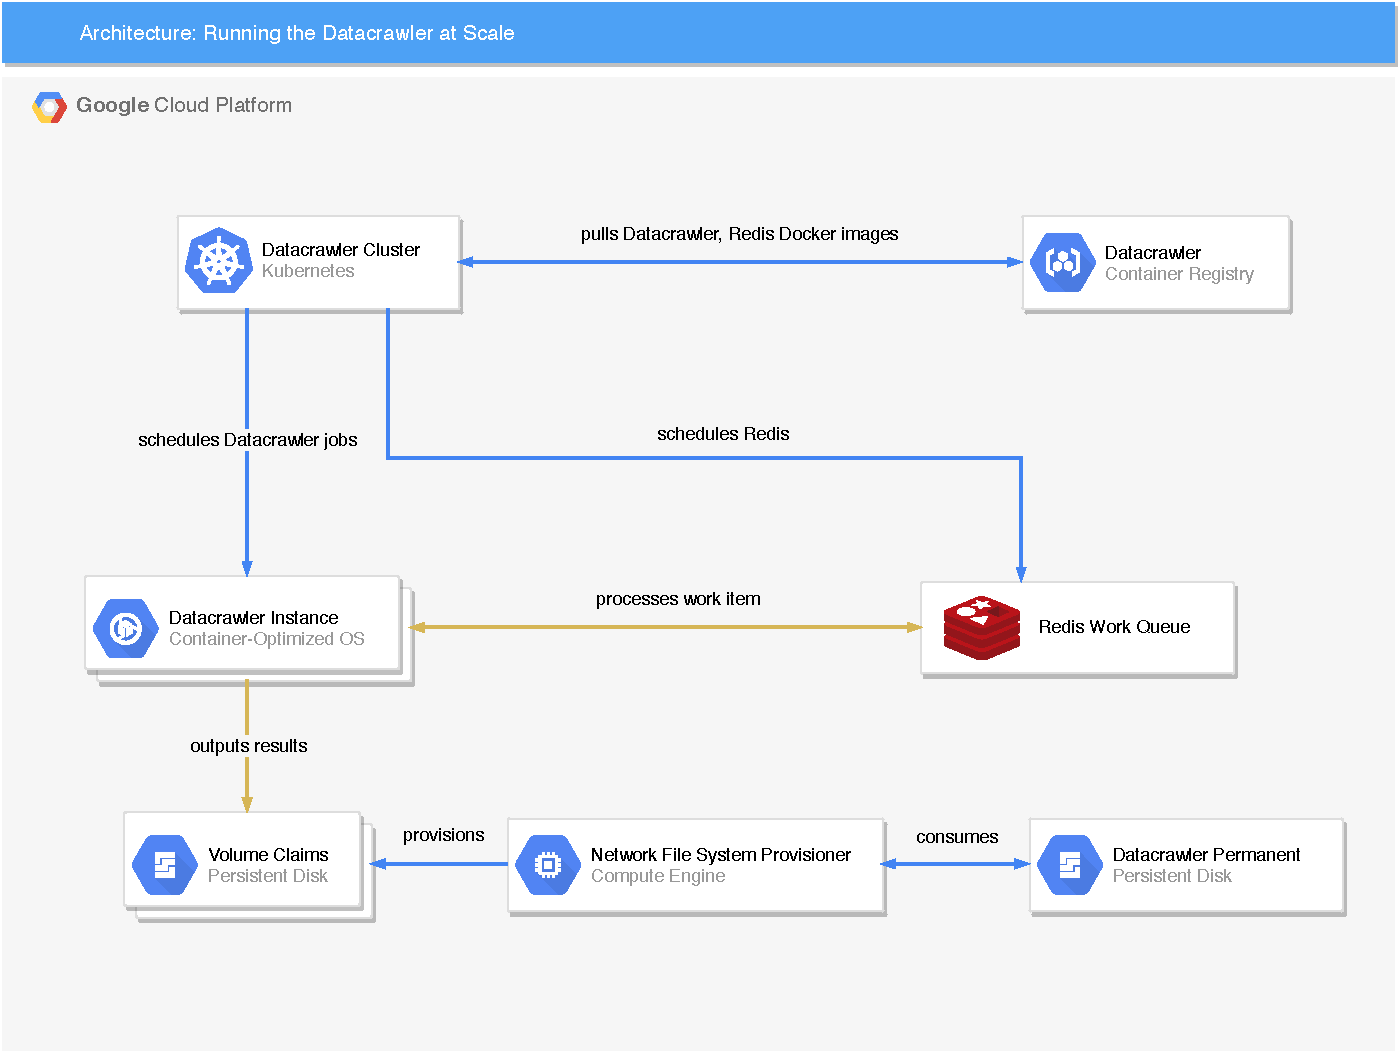
\includegraphics[scale=0.5]{resources/datacrawler_k8s_architecture}
	\caption[System Design of "Running the Datacrawler at Scale"]{Illustration of the system design of the Datacrawler Kubernetes cluster on Google Cloud Platform. It shows that the Datacrawler Kubernetes cluster consists mainly out of three applications: The \texttt{redis}-queue which represents a work queue consisting out of domains as work items to be analyzed. The Network File System provisioner which is mainly responsible for providing volume claims for Datacrawler instances from the central storage. Finally, the Datacrawler which is deployed as a container from the internal Docker registry. The Datacrawler itself is executed wrapped by a \texttt{python}-application, which represents the tie between the \texttt{redis}-queue and the Datacrawler. It is resposible for retrieving of work items from the queue, starting the Datacrawler and confirming the work item upon successful analysis.}
	\label{datacrawler_k8s_architecture}
\end{figure}
\paragraph*{Datacrawler as a Container}
\label{datacrawler_container}

As discussed in earlier sections, Kubernetes is only able to schedule containers, not directly applications such as our Datacrawler. Simply illustrated a container represents an isolated subsystem of the host system where it is run. In contrast to a virtual machine, a container shares the same hardware and kernel of the host system. The isolation consists of isolating processes from the host system to the container and vice versa. Within a container the user is able to run multiple applications as he would do usual on the host system. 

The Datacrawler container is created during the deployment by the Kubernetes cluster from a custom Docker image, which can be found in our internal Docker registry in Google Cloud Platform. We locally build the Datacrawler for \texttt{Linux}, pack it to a \texttt{Linux} Docker image on our local development machine and push it our internal Docker registry on Google Cloud Platform. 

Upon we request the deployment of $100$ Datacrawler instances, Kubernetes tries to allocate the resources required per Datacrawler. We define those requirements within the request. In our case if Kubernetes fails to allocate required resources, it automatically provisions new compute nodes to deploy the Datacrawler until the deployment is successful. Upon successful allocation, Kubernetes requests and mounts a volume from the NFS provisioner to \texttt{/opt/apt/datacrawler-data/}, which represents the location where results should be saved to. Afterwards the container is being started with the \texttt{Python}-file \texttt{worker.py} as entrypoint. \texttt{worker.py} is mainly responsible to be the tie between the \texttt{redis} work queue and the Datacrawler instances. It connects with the \texttt{redis}-instance in the cluster, accepts new working items, starts a Datacrawler instance for each work item and passes the rank and domain using environment variables to the Datacrawler. Upon the Datacrawler successfully exits, confirms the work item and removes it from our working queue. We repeat this until the working queue is empty.

\subsubsection{Datacrawler Evaluation}
\label{datacrawler_results}
The main goal of the Datacrawler was to generate dataset version 1 and 2 according to the specifications described in Section~\ref{DatasetVersion1} and \ref{DatasetVersion2} respectively. During the runs of the Datacrawler, we faced serious difficulties in running the Datacrawler stable at scale. It required multiple restarts for both dataset versions to crawl $100,000$ domains given by our ground truth Open PageRank (Section~\ref{OpenPageRank}).

In fact local experiments showed that we were successfully able to scale the Datacrawler and crawl a subset of domains for both dataset versions (100 domains à 10 Datacrawler instances) without using Kubernetes and a working queue. The results of our local experiments unfortunately did not reflect our results in Kubernetes on Google Cloud Platform. In both dataset versions the \texttt{redis} working queue was unstable due to the large amount of incoming requests. It occasionally crashed and stopped the whole crawling process. Unfortunately, we were not able to find the root cause in the given short time frame, therefore we sticked to our approach watch-and-restart until we crawled all given domains.

In addition to our working queue, the Datacrawler has also shown instabilities regarding the generation of the mobile and desktop screenshots. In average 10 - 15 \% of the domains the Datacrawler delivered black or white screenshots. We strongly assume that this is solely caused by malfunction of the Datacrawler. We answered this occurrence by analyzing all samples in both datasets and removing all domains having only black and white screenshots. We strongly assume that the removal has little impact on our research.

In the end, the Datacrawler has delivered 83296 valid samples for dataset version 1 and 87629 valid samples for dataset version 2.